\documentclass{book}
\usepackage[a4paper,top=2.5cm,bottom=2.5cm,left=2.5cm,right=2.5cm]{geometry}
\usepackage{makeidx}
\usepackage{natbib}
\usepackage{graphicx}
\usepackage{multicol}
\usepackage{float}
\usepackage{listings}
\usepackage{color}
\usepackage{ifthen}
\usepackage[table]{xcolor}
\usepackage{textcomp}
\usepackage{alltt}
\usepackage{ifpdf}
\ifpdf
\usepackage[pdftex,
            pagebackref=true,
            colorlinks=true,
            linkcolor=blue,
            unicode
           ]{hyperref}
\else
\usepackage[ps2pdf,
            pagebackref=true,
            colorlinks=true,
            linkcolor=blue,
            unicode
           ]{hyperref}
\usepackage{pspicture}
\fi
\usepackage[utf8]{inputenc}
\usepackage{mathptmx}
\usepackage[scaled=.90]{helvet}
\usepackage{courier}
\usepackage{sectsty}
\usepackage{amssymb}
\usepackage[titles]{tocloft}
\usepackage{doxygen}
\lstset{language=C++,inputencoding=utf8,basicstyle=\footnotesize,breaklines=true,breakatwhitespace=true,tabsize=4,numbers=left }
\makeindex
\setcounter{tocdepth}{3}
\renewcommand{\footrulewidth}{0.4pt}
\renewcommand{\familydefault}{\sfdefault}
\hfuzz=15pt
\setlength{\emergencystretch}{15pt}
\hbadness=750
\tolerance=750
\begin{document}
\hypersetup{pageanchor=false,citecolor=blue}
\begin{titlepage}
\vspace*{7cm}
\begin{center}
{\Large Nooba Plugin A\-P\-I \\[1ex]\large 0.\-12 }\\
\vspace*{1cm}
{\large Generated by Doxygen 1.8.3.1}\\
\vspace*{0.5cm}
{\small Sat Dec 7 2013 09:59:04}\\
\end{center}
\end{titlepage}
\clearemptydoublepage
\pagenumbering{roman}
\tableofcontents
\clearemptydoublepage
\pagenumbering{arabic}
\hypersetup{pageanchor=true,citecolor=blue}
\chapter{Namespace Index}
\section{Namespace List}
Here is a list of all documented namespaces with brief descriptions\-:\begin{DoxyCompactList}
\item\contentsline{section}{\hyperlink{namespacenooba}{nooba} \\*Nooba namespace }{\pageref{namespacenooba}}{}
\end{DoxyCompactList}

\chapter{Hierarchical Index}
\section{Class Hierarchy}
This inheritance list is sorted roughly, but not completely, alphabetically\-:\begin{DoxyCompactList}
\item \contentsline{section}{Nooba\-Plugin\-A\-P\-I\-Base\-Private}{\pageref{class_nooba_plugin_a_p_i_base_private}}{}
\item \contentsline{section}{Nooba\-Plugin\-A\-P\-I\-Private}{\pageref{struct_nooba_plugin_a_p_i_private}}{}
\item \contentsline{section}{Plugin\-Info}{\pageref{class_plugin_info}}{}
\item \contentsline{section}{Plugin\-Info\-Private}{\pageref{struct_plugin_info_private}}{}
\item \contentsline{section}{Plugin\-Pass\-Data}{\pageref{class_plugin_pass_data}}{}
\item \contentsline{section}{Plugin\-Pass\-Data\-Private}{\pageref{struct_plugin_pass_data_private}}{}
\item \contentsline{section}{Proc\-Params}{\pageref{class_proc_params}}{}
\item \contentsline{section}{Proc\-Params\-Private}{\pageref{struct_proc_params_private}}{}
\item Q\-Object\begin{DoxyCompactList}
\item \contentsline{section}{Nooba\-Plugin\-A\-P\-I\-Base}{\pageref{class_nooba_plugin_a_p_i_base}}{}
\begin{DoxyCompactList}
\item \contentsline{section}{Nooba\-Plugin\-A\-P\-I}{\pageref{class_nooba_plugin_a_p_i}}{}
\end{DoxyCompactList}
\end{DoxyCompactList}
\end{DoxyCompactList}

\chapter{Class Index}
\section{Class List}
Here are the classes, structs, unions and interfaces with brief descriptions\-:\begin{DoxyCompactList}
\item\contentsline{section}{\hyperlink{class_nooba_plugin_a_p_i}{Nooba\-Plugin\-A\-P\-I} }{\pageref{class_nooba_plugin_a_p_i}}{}
\item\contentsline{section}{\hyperlink{class_nooba_plugin_a_p_i_base}{Nooba\-Plugin\-A\-P\-I\-Base} }{\pageref{class_nooba_plugin_a_p_i_base}}{}
\item\contentsline{section}{\hyperlink{class_nooba_plugin_a_p_i_base_private}{Nooba\-Plugin\-A\-P\-I\-Base\-Private} }{\pageref{class_nooba_plugin_a_p_i_base_private}}{}
\item\contentsline{section}{\hyperlink{struct_nooba_plugin_a_p_i_private}{Nooba\-Plugin\-A\-P\-I\-Private} \\*The \hyperlink{struct_nooba_plugin_a_p_i_private}{Nooba\-Plugin\-A\-P\-I\-Private} struct private data structure for \hyperlink{class_nooba_plugin_a_p_i}{Nooba\-Plugin\-A\-P\-I} class }{\pageref{struct_nooba_plugin_a_p_i_private}}{}
\item\contentsline{section}{\hyperlink{class_plugin_info}{Plugin\-Info} \\*Plugin information are stored in this structure }{\pageref{class_plugin_info}}{}
\item\contentsline{section}{\hyperlink{struct_plugin_info_private}{Plugin\-Info\-Private} }{\pageref{struct_plugin_info_private}}{}
\item\contentsline{section}{\hyperlink{class_plugin_pass_data}{Plugin\-Pass\-Data} }{\pageref{class_plugin_pass_data}}{}
\item\contentsline{section}{\hyperlink{struct_plugin_pass_data_private}{Plugin\-Pass\-Data\-Private} \\*The \hyperlink{struct_plugin_pass_data_private}{Plugin\-Pass\-Data\-Private} struct }{\pageref{struct_plugin_pass_data_private}}{}
\item\contentsline{section}{\hyperlink{class_proc_params}{Proc\-Params} \\*Structure that uses to pass frame relevant data from the Frontend application to base plugin }{\pageref{class_proc_params}}{}
\item\contentsline{section}{\hyperlink{struct_proc_params_private}{Proc\-Params\-Private} }{\pageref{struct_proc_params_private}}{}
\end{DoxyCompactList}

\chapter{Namespace Documentation}
\hypertarget{namespacenooba}{\section{nooba Namespace Reference}
\label{namespacenooba}\index{nooba@{nooba}}
}


Nooba namespace.  


\subsection*{Enumerations}
\begin{DoxyCompactItemize}
\item 
enum \hyperlink{namespacenooba_ac8cd2c91afc9699430b5db4d0d257587}{Param\-Type} \{ \\*
\hyperlink{namespacenooba_ac8cd2c91afc9699430b5db4d0d257587aba76ac90ab7d88718d47c2ad438b4174}{Int\-Param} = 0, 
\hyperlink{namespacenooba_ac8cd2c91afc9699430b5db4d0d257587a7a9f0f2aeb74323c2831d34b081ebae7}{Double\-Param} = 1, 
\hyperlink{namespacenooba_ac8cd2c91afc9699430b5db4d0d257587a9075ba9755692c2db8f88280744ec213}{String\-Param} = 2, 
\hyperlink{namespacenooba_ac8cd2c91afc9699430b5db4d0d257587a6002a3a125d72a8c57bee6fc0349ccb5}{Range\-Param} = 3, 
\\*
\hyperlink{namespacenooba_ac8cd2c91afc9699430b5db4d0d257587a3ef63c5bcb93e80fcea79b4a53356a7a}{Region\-Param} = 4, 
\hyperlink{namespacenooba_ac8cd2c91afc9699430b5db4d0d257587af7aec3247e179b6803ec617efafccb5a}{Multi\-Value\-Param} = 5, 
\hyperlink{namespacenooba_ac8cd2c91afc9699430b5db4d0d257587aa4c781f429d7130738a337576be3cd7a}{File\-Path\-Param} = 6
 \}
\begin{DoxyCompactList}\small\item\em Parameter type enum. \end{DoxyCompactList}\item 
enum \hyperlink{namespacenooba_ae2951593fff55d4ea388efa06a663468}{Video\-State} \{ \hyperlink{namespacenooba_ae2951593fff55d4ea388efa06a663468a2f89a7c81cc705e85b32af68710d9825}{Playing\-State} = 0, 
\hyperlink{namespacenooba_ae2951593fff55d4ea388efa06a663468a6a2fd6bf8ba2b19fb47d8d4fcfb0ee04}{Paused\-State} = 1, 
\hyperlink{namespacenooba_ae2951593fff55d4ea388efa06a663468abdc20322ae46c842f82b4445256904fe}{Stopped\-State} = 2
 \}
\begin{DoxyCompactList}\small\item\em The Video\-State enum. \end{DoxyCompactList}\item 
enum \hyperlink{namespacenooba_a1e392455e0e2d24934ea87baaf5eb43c}{Alert\-Type} \{ \hyperlink{namespacenooba_a1e392455e0e2d24934ea87baaf5eb43ca711484b17f4df008c92858ee6b78cfe2}{Red\-Alert} = 0, 
\hyperlink{namespacenooba_a1e392455e0e2d24934ea87baaf5eb43ca1f227410c59654b49512f1926f19ef29}{Amber\-Alert} = 1
 \}
\begin{DoxyCompactList}\small\item\em The Alert\-Type enum. \end{DoxyCompactList}\item 
enum \hyperlink{namespacenooba_a63ed48aaaaeaf49835daddab6c63695e}{Path\-Type} \{ \hyperlink{namespacenooba_a63ed48aaaaeaf49835daddab6c63695eaf95e834f706cf854b89935b78de070bd}{File\-Path} = 0, 
\hyperlink{namespacenooba_a63ed48aaaaeaf49835daddab6c63695eac506ef2b72e507e01d1365c73dee614b}{Dir\-Path} = 1
 \}
\begin{DoxyCompactList}\small\item\em The Path\-Type enum. \end{DoxyCompactList}\end{DoxyCompactItemize}


\subsection{Detailed Description}
Nooba namespace. This namespace contains the identifiers used by the \hyperlink{class_nooba_plugin_a_p_i}{Nooba\-Plugin\-A\-P\-I}. Different enum types used 

\subsection{Enumeration Type Documentation}
\hypertarget{namespacenooba_a1e392455e0e2d24934ea87baaf5eb43c}{\index{nooba@{nooba}!Alert\-Type@{Alert\-Type}}
\index{Alert\-Type@{Alert\-Type}!nooba@{nooba}}
\subsubsection[{Alert\-Type}]{\setlength{\rightskip}{0pt plus 5cm}enum {\bf nooba\-::\-Alert\-Type}}}\label{namespacenooba_a1e392455e0e2d24934ea87baaf5eb43c}


The Alert\-Type enum. 

These are the type of alert levels identified by the system. These alert level can be generated by calling \hyperlink{class_nooba_plugin_a_p_i_a643a07495d139b132bf52a27dda6ff09}{Nooba\-Plugin\-A\-P\-I\-::generate\-Alert}(...) function \begin{DoxySeeAlso}{See Also}
\hyperlink{class_nooba_plugin_a_p_i_a643a07495d139b132bf52a27dda6ff09}{Nooba\-Plugin\-A\-P\-I\-::generate\-Alert()} 
\end{DoxySeeAlso}
\begin{Desc}
\item[Enumerator]\par
\begin{description}
\index{Red\-Alert@{Red\-Alert}!nooba@{nooba}}\index{nooba@{nooba}!Red\-Alert@{Red\-Alert}}\item[{\em 
\hypertarget{namespacenooba_a1e392455e0e2d24934ea87baaf5eb43ca711484b17f4df008c92858ee6b78cfe2}{Red\-Alert}\label{namespacenooba_a1e392455e0e2d24934ea87baaf5eb43ca711484b17f4df008c92858ee6b78cfe2}
}]Highest priority alert, alert level 0 \index{Amber\-Alert@{Amber\-Alert}!nooba@{nooba}}\index{nooba@{nooba}!Amber\-Alert@{Amber\-Alert}}\item[{\em 
\hypertarget{namespacenooba_a1e392455e0e2d24934ea87baaf5eb43ca1f227410c59654b49512f1926f19ef29}{Amber\-Alert}\label{namespacenooba_a1e392455e0e2d24934ea87baaf5eb43ca1f227410c59654b49512f1926f19ef29}
}]Secenod most important alert, alert level 1 \end{description}
\end{Desc}
\hypertarget{namespacenooba_ac8cd2c91afc9699430b5db4d0d257587}{\index{nooba@{nooba}!Param\-Type@{Param\-Type}}
\index{Param\-Type@{Param\-Type}!nooba@{nooba}}
\subsubsection[{Param\-Type}]{\setlength{\rightskip}{0pt plus 5cm}enum {\bf nooba\-::\-Param\-Type}}}\label{namespacenooba_ac8cd2c91afc9699430b5db4d0d257587}


Parameter type enum. 

Parameter types used in Nooba V\-S\-S system is defined here. \begin{Desc}
\item[Enumerator]\par
\begin{description}
\index{Int\-Param@{Int\-Param}!nooba@{nooba}}\index{nooba@{nooba}!Int\-Param@{Int\-Param}}\item[{\em 
\hypertarget{namespacenooba_ac8cd2c91afc9699430b5db4d0d257587aba76ac90ab7d88718d47c2ad438b4174}{Int\-Param}\label{namespacenooba_ac8cd2c91afc9699430b5db4d0d257587aba76ac90ab7d88718d47c2ad438b4174}
}]Integer parameter \index{Double\-Param@{Double\-Param}!nooba@{nooba}}\index{nooba@{nooba}!Double\-Param@{Double\-Param}}\item[{\em 
\hypertarget{namespacenooba_ac8cd2c91afc9699430b5db4d0d257587a7a9f0f2aeb74323c2831d34b081ebae7}{Double\-Param}\label{namespacenooba_ac8cd2c91afc9699430b5db4d0d257587a7a9f0f2aeb74323c2831d34b081ebae7}
}]Double parameter to be used in parameters that need double precision \index{String\-Param@{String\-Param}!nooba@{nooba}}\index{nooba@{nooba}!String\-Param@{String\-Param}}\item[{\em 
\hypertarget{namespacenooba_ac8cd2c91afc9699430b5db4d0d257587a9075ba9755692c2db8f88280744ec213}{String\-Param}\label{namespacenooba_ac8cd2c91afc9699430b5db4d0d257587a9075ba9755692c2db8f88280744ec213}
}]To take string variables as input \index{Range\-Param@{Range\-Param}!nooba@{nooba}}\index{nooba@{nooba}!Range\-Param@{Range\-Param}}\item[{\em 
\hypertarget{namespacenooba_ac8cd2c91afc9699430b5db4d0d257587a6002a3a125d72a8c57bee6fc0349ccb5}{Range\-Param}\label{namespacenooba_ac8cd2c91afc9699430b5db4d0d257587a6002a3a125d72a8c57bee6fc0349ccb5}
}]Integer parameter \index{Region\-Param@{Region\-Param}!nooba@{nooba}}\index{nooba@{nooba}!Region\-Param@{Region\-Param}}\item[{\em 
\hypertarget{namespacenooba_ac8cd2c91afc9699430b5db4d0d257587a3ef63c5bcb93e80fcea79b4a53356a7a}{Region\-Param}\label{namespacenooba_ac8cd2c91afc9699430b5db4d0d257587a3ef63c5bcb93e80fcea79b4a53356a7a}
}]Parameter defining Region of Interest \index{Multi\-Value\-Param@{Multi\-Value\-Param}!nooba@{nooba}}\index{nooba@{nooba}!Multi\-Value\-Param@{Multi\-Value\-Param}}\item[{\em 
\hypertarget{namespacenooba_ac8cd2c91afc9699430b5db4d0d257587af7aec3247e179b6803ec617efafccb5a}{Multi\-Value\-Param}\label{namespacenooba_ac8cd2c91afc9699430b5db4d0d257587af7aec3247e179b6803ec617efafccb5a}
}]Parameter where multiple predefined values are given to user to choose from \index{File\-Path\-Param@{File\-Path\-Param}!nooba@{nooba}}\index{nooba@{nooba}!File\-Path\-Param@{File\-Path\-Param}}\item[{\em 
\hypertarget{namespacenooba_ac8cd2c91afc9699430b5db4d0d257587aa4c781f429d7130738a337576be3cd7a}{File\-Path\-Param}\label{namespacenooba_ac8cd2c91afc9699430b5db4d0d257587aa4c781f429d7130738a337576be3cd7a}
}]File paths are taken as input through this parameters \end{description}
\end{Desc}
\hypertarget{namespacenooba_a63ed48aaaaeaf49835daddab6c63695e}{\index{nooba@{nooba}!Path\-Type@{Path\-Type}}
\index{Path\-Type@{Path\-Type}!nooba@{nooba}}
\subsubsection[{Path\-Type}]{\setlength{\rightskip}{0pt plus 5cm}enum {\bf nooba\-::\-Path\-Type}}}\label{namespacenooba_a63ed48aaaaeaf49835daddab6c63695e}


The Path\-Type enum. 

In some cases different types of paths need to be selected. This enum difines the supported path types by the system \begin{Desc}
\item[Enumerator]\par
\begin{description}
\index{File\-Path@{File\-Path}!nooba@{nooba}}\index{nooba@{nooba}!File\-Path@{File\-Path}}\item[{\em 
\hypertarget{namespacenooba_a63ed48aaaaeaf49835daddab6c63695eaf95e834f706cf854b89935b78de070bd}{File\-Path}\label{namespacenooba_a63ed48aaaaeaf49835daddab6c63695eaf95e834f706cf854b89935b78de070bd}
}]Single file path \index{Dir\-Path@{Dir\-Path}!nooba@{nooba}}\index{nooba@{nooba}!Dir\-Path@{Dir\-Path}}\item[{\em 
\hypertarget{namespacenooba_a63ed48aaaaeaf49835daddab6c63695eac506ef2b72e507e01d1365c73dee614b}{Dir\-Path}\label{namespacenooba_a63ed48aaaaeaf49835daddab6c63695eac506ef2b72e507e01d1365c73dee614b}
}]Single Directory path \end{description}
\end{Desc}
\hypertarget{namespacenooba_ae2951593fff55d4ea388efa06a663468}{\index{nooba@{nooba}!Video\-State@{Video\-State}}
\index{Video\-State@{Video\-State}!nooba@{nooba}}
\subsubsection[{Video\-State}]{\setlength{\rightskip}{0pt plus 5cm}enum {\bf nooba\-::\-Video\-State}}}\label{namespacenooba_ae2951593fff55d4ea388efa06a663468}


The Video\-State enum. 

This enum defines the current video state of the system. Whether the video stream is playing, paused or stopped. \begin{Desc}
\item[Enumerator]\par
\begin{description}
\index{Playing\-State@{Playing\-State}!nooba@{nooba}}\index{nooba@{nooba}!Playing\-State@{Playing\-State}}\item[{\em 
\hypertarget{namespacenooba_ae2951593fff55d4ea388efa06a663468a2f89a7c81cc705e85b32af68710d9825}{Playing\-State}\label{namespacenooba_ae2951593fff55d4ea388efa06a663468a2f89a7c81cc705e85b32af68710d9825}
}]video playing State \index{Paused\-State@{Paused\-State}!nooba@{nooba}}\index{nooba@{nooba}!Paused\-State@{Paused\-State}}\item[{\em 
\hypertarget{namespacenooba_ae2951593fff55d4ea388efa06a663468a6a2fd6bf8ba2b19fb47d8d4fcfb0ee04}{Paused\-State}\label{namespacenooba_ae2951593fff55d4ea388efa06a663468a6a2fd6bf8ba2b19fb47d8d4fcfb0ee04}
}]Video paused State \index{Stopped\-State@{Stopped\-State}!nooba@{nooba}}\index{nooba@{nooba}!Stopped\-State@{Stopped\-State}}\item[{\em 
\hypertarget{namespacenooba_ae2951593fff55d4ea388efa06a663468abdc20322ae46c842f82b4445256904fe}{Stopped\-State}\label{namespacenooba_ae2951593fff55d4ea388efa06a663468abdc20322ae46c842f82b4445256904fe}
}]video stopped State \end{description}
\end{Desc}

\chapter{Class Documentation}
\hypertarget{class_nooba_plugin_a_p_i}{\section{Nooba\-Plugin\-A\-P\-I Class Reference}
\label{class_nooba_plugin_a_p_i}\index{Nooba\-Plugin\-A\-P\-I@{Nooba\-Plugin\-A\-P\-I}}
}
Inheritance diagram for Nooba\-Plugin\-A\-P\-I\-:\begin{figure}[H]
\begin{center}
\leavevmode
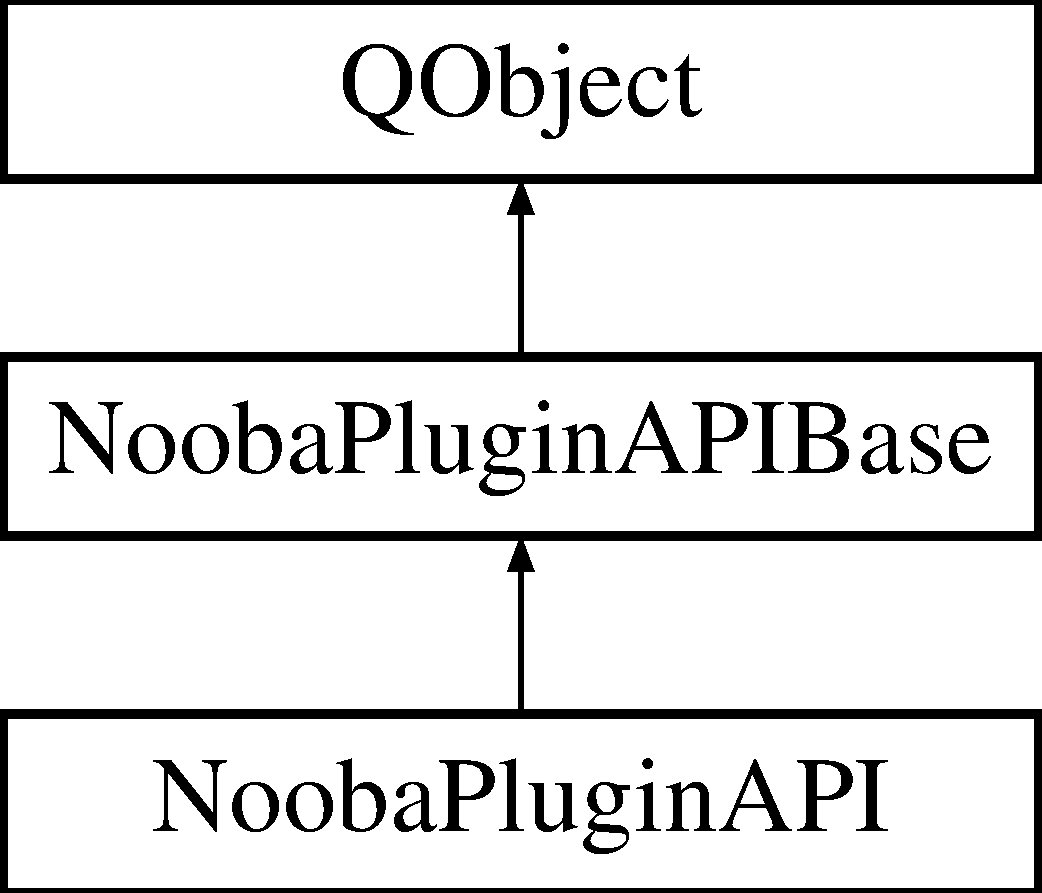
\includegraphics[height=3.000000cm]{class_nooba_plugin_a_p_i}
\end{center}
\end{figure}
\subsection*{Public Slots}
\begin{DoxyCompactItemize}
\item 
virtual void \hyperlink{class_nooba_plugin_a_p_i_a1c6dfbd25f56949f058f2ec1c778c255}{on\-Int\-Param\-Changed} (const Q\-String \&var\-Name, int val)
\item 
\hypertarget{class_nooba_plugin_a_p_i_a943eecd58855dce164b2ee772f821cc4}{virtual void {\bfseries on\-Double\-Param\-Changed} (const Q\-String \&var\-Name, double val)}\label{class_nooba_plugin_a_p_i_a943eecd58855dce164b2ee772f821cc4}

\item 
\hypertarget{class_nooba_plugin_a_p_i_a27b9c788c723dfc7f65c89df28fd72f6}{virtual void {\bfseries on\-String\-Param\-Changed} (const Q\-String \&var\-Name, const Q\-String \&val)}\label{class_nooba_plugin_a_p_i_a27b9c788c723dfc7f65c89df28fd72f6}

\item 
\hypertarget{class_nooba_plugin_a_p_i_adc036b89ba60176bb22be9c57ba928dc}{virtual void {\bfseries on\-Multi\-Val\-Param\-Changed} (const Q\-String \&var\-Name, const Q\-String \&val)}\label{class_nooba_plugin_a_p_i_adc036b89ba60176bb22be9c57ba928dc}

\item 
\hypertarget{class_nooba_plugin_a_p_i_a424cc229b473f03569b62c467d593b0a}{virtual void {\bfseries on\-File\-Path\-Param\-Changed} (const Q\-String \&var\-Name, const Q\-String \&path)}\label{class_nooba_plugin_a_p_i_a424cc229b473f03569b62c467d593b0a}

\item 
virtual void \hyperlink{class_nooba_plugin_a_p_i_a1957f0d0dd3820bc612bf718c4563f3c}{input\-Data} (const \hyperlink{class_plugin_pass_data}{Plugin\-Pass\-Data} \&data)
\begin{DoxyCompactList}\small\item\em input\-Data data received from other plugin thru thid function. This is used to interconnect plugins. Another plugins output\-Data(\-Plugin\-Pass\-Data$\ast$ data) can be connected to this slot. \end{DoxyCompactList}\item 
\hypertarget{class_nooba_plugin_a_p_i_a76b29ea195cae378ab04de715212a00e}{virtual void {\bfseries input\-Data} (const Q\-String\-List \&str\-List, Q\-List$<$ Q\-Image $>$ image\-List)}\label{class_nooba_plugin_a_p_i_a76b29ea195cae378ab04de715212a00e}

\item 
\hypertarget{class_nooba_plugin_a_p_i_a312e1f7842db25aed043e8fee07e644f}{virtual void {\bfseries on\-Line\-Param\-Updated} (const Q\-String \&var\-Name, const Q\-String frame\-Viewer\-Title, Q\-Line line)}\label{class_nooba_plugin_a_p_i_a312e1f7842db25aed043e8fee07e644f}

\end{DoxyCompactItemize}
\subsection*{Signals}
\begin{DoxyCompactItemize}
\item 
\hypertarget{class_nooba_plugin_a_p_i_a7ca475f8be6c10a6f0f3bc9b5f8076be}{void {\bfseries create\-Int\-Param\-Request} (const Q\-String \&var\-Name, int val, int max=100, int min=0)}\label{class_nooba_plugin_a_p_i_a7ca475f8be6c10a6f0f3bc9b5f8076be}

\item 
\hypertarget{class_nooba_plugin_a_p_i_a2c798592fda37a108b9b141688904502}{void {\bfseries create\-Double\-Param\-Request} (const Q\-String \&var\-Name, double val, double max=100.\-0, double min=0.\-0)}\label{class_nooba_plugin_a_p_i_a2c798592fda37a108b9b141688904502}

\item 
\hypertarget{class_nooba_plugin_a_p_i_aace29b22ace007cd11d920a1f4ca7c86}{void {\bfseries create\-String\-Param\-Request} (const Q\-String \&var\-Name, Q\-String val, bool is\-File\-Path=false)}\label{class_nooba_plugin_a_p_i_aace29b22ace007cd11d920a1f4ca7c86}

\item 
\hypertarget{class_nooba_plugin_a_p_i_a7a30dd6d87281b1bdaa8e63c3277c09f}{void {\bfseries create\-Multi\-Val\-Param\-Request} (const Q\-String \&var\-Name, const Q\-String\-List \&var\-List)}\label{class_nooba_plugin_a_p_i_a7a30dd6d87281b1bdaa8e63c3277c09f}

\item 
\hypertarget{class_nooba_plugin_a_p_i_a8e491471624e53dc54b36fe16a38749a}{void {\bfseries create\-Line\-Param\-Request} (const Q\-String \&var\-Name, const Q\-String \&frame\-Viewer\-Title, Q\-Color line\-Color)}\label{class_nooba_plugin_a_p_i_a8e491471624e53dc54b36fe16a38749a}

\item 
\hypertarget{class_nooba_plugin_a_p_i_a70ebb0070b79b33737532162b682a8a5}{void {\bfseries debug\-Msg\-Request} (const Q\-String \&msg)}\label{class_nooba_plugin_a_p_i_a70ebb0070b79b33737532162b682a8a5}

\item 
\hypertarget{class_nooba_plugin_a_p_i_a707c8e8219f628535fb5155a7782df1d}{void {\bfseries output\-Data\-Request} (const \hyperlink{class_plugin_pass_data}{Plugin\-Pass\-Data} \&data)}\label{class_nooba_plugin_a_p_i_a707c8e8219f628535fb5155a7782df1d}

\item 
\hypertarget{class_nooba_plugin_a_p_i_aec28bddd8844b426d781eec2d77aa3d0}{void {\bfseries output\-Data\-Request} (const Q\-String\-List \&str\-List, Q\-List$<$ Q\-Image $>$ image\-List)}\label{class_nooba_plugin_a_p_i_aec28bddd8844b426d781eec2d77aa3d0}

\item 
\hypertarget{class_nooba_plugin_a_p_i_a52a0aae14f9ee31427409868a8014ee9}{void {\bfseries create\-Frame\-Viewer\-Request} (const Q\-String \&title, bool is\-Visible=true)}\label{class_nooba_plugin_a_p_i_a52a0aae14f9ee31427409868a8014ee9}

\item 
\hypertarget{class_nooba_plugin_a_p_i_a5716225fae1e93b57ab623fab6e509b8}{void {\bfseries update\-Frame\-Viewer\-Request} (const Q\-String \&title, const Q\-Image \&frame)}\label{class_nooba_plugin_a_p_i_a5716225fae1e93b57ab623fab6e509b8}

\item 
\hypertarget{class_nooba_plugin_a_p_i_a5918fa3bc2b6ec19f632783010b357cc}{void {\bfseries update\-Frame\-Viewer\-Visibility\-Request} (const Q\-String \&title, bool is\-Visible)}\label{class_nooba_plugin_a_p_i_a5918fa3bc2b6ec19f632783010b357cc}

\item 
\hypertarget{class_nooba_plugin_a_p_i_ac28438c24ca60e790eabf1c97c8dedbc}{void {\bfseries create\-File\-Path\-Param\-Request} (const Q\-String \&var\-Name, Q\-String path, \hyperlink{namespacenooba_a63ed48aaaaeaf49835daddab6c63695e}{nooba\-::\-Path\-Type} path\-Type, const Q\-String \&filter)}\label{class_nooba_plugin_a_p_i_ac28438c24ca60e790eabf1c97c8dedbc}

\item 
\hypertarget{class_nooba_plugin_a_p_i_a1c5091983135dea3d45050600e8b1b73}{void {\bfseries generate\-Alert\-Request} (const Q\-String \&frame\-Viewer\-Title, const Q\-String \&msg, \hyperlink{namespacenooba_a1e392455e0e2d24934ea87baaf5eb43c}{nooba\-::\-Alert\-Type} alert)}\label{class_nooba_plugin_a_p_i_a1c5091983135dea3d45050600e8b1b73}

\end{DoxyCompactItemize}
\subsection*{Public Member Functions}
\begin{DoxyCompactItemize}
\item 
virtual bool \hyperlink{class_nooba_plugin_a_p_i_a213d0b72183f3266397529925fe57466}{init} ()=0
\begin{DoxyCompactList}\small\item\em Initialise the resources used by the Plugin. \end{DoxyCompactList}\item 
virtual bool \hyperlink{class_nooba_plugin_a_p_i_a2b0532499d63ed3f29ab9ab5bf4caebe}{release} ()=0
\begin{DoxyCompactList}\small\item\em releases the resources used by the plugin. \end{DoxyCompactList}\item 
virtual bool \hyperlink{class_nooba_plugin_a_p_i_ac3878e3576fcc7ca5fbcc111355d2a49}{proc\-Frame} (const cv\-::\-Mat \&in, cv\-::\-Mat \&out, \hyperlink{class_proc_params}{Proc\-Params} \&params)=0
\begin{DoxyCompactList}\small\item\em Base plugins' processing is done by calling this function. \end{DoxyCompactList}\item 
virtual \hyperlink{class_plugin_info}{Plugin\-Info} \hyperlink{class_nooba_plugin_a_p_i_a1d616b65830b222f8ffa4ed374ae6f15}{get\-Plugin\-Info} () const =0
\begin{DoxyCompactList}\small\item\em metadata related to the plugin is taken from the function \end{DoxyCompactList}\item 
void \hyperlink{class_nooba_plugin_a_p_i_ab01db814b095792dd5eff8d91804b50b}{create\-Int\-Param} (const Q\-String \&var\-Name, int val, int max=100, int min=0)
\begin{DoxyCompactList}\small\item\em integer parameters can be created using this function \end{DoxyCompactList}\item 
void \hyperlink{class_nooba_plugin_a_p_i_ae0d8554682787f936739b33e9e4c1191}{create\-Double\-Param} (const Q\-String \&var\-Name, double val, double max=100.\-0, double min=0.\-0)
\begin{DoxyCompactList}\small\item\em double parameters can be created using this function \end{DoxyCompactList}\item 
void \hyperlink{class_nooba_plugin_a_p_i_adeb3d73461908d5bc4b0e2749ec9a74e}{create\-String\-Param} (const Q\-String \&var\-Name, Q\-String val, bool is\-File\-Path=false)
\begin{DoxyCompactList}\small\item\em String parameters can be created using this function. \end{DoxyCompactList}\item 
void \hyperlink{class_nooba_plugin_a_p_i_af2517b4c6e3c48d38cf9dd7667a03186}{create\-File\-Path\-Param} (const Q\-String \&var\-Name, Q\-String path=Q\-String(), \hyperlink{namespacenooba_a63ed48aaaaeaf49835daddab6c63695e}{nooba\-::\-Path\-Type} path\-Type=\hyperlink{namespacenooba_a63ed48aaaaeaf49835daddab6c63695eaf95e834f706cf854b89935b78de070bd}{nooba\-::\-File\-Path}, const Q\-String \&filter=Q\-String())
\begin{DoxyCompactList}\small\item\em file\-Path parameters can be created using this function \end{DoxyCompactList}\item 
void \hyperlink{class_nooba_plugin_a_p_i_a210a3566212cc6ca1e947a8b8bec3818}{create\-Multi\-Val\-Param} (const Q\-String \&var\-Name, const Q\-String\-List \&var\-List)
\begin{DoxyCompactList}\small\item\em Multi value Parameters can be created using this function. \end{DoxyCompactList}\item 
void \hyperlink{class_nooba_plugin_a_p_i_a144f4a7f58fb393cab86d7b90d4a4728}{create\-Line\-Param} (const Q\-String \&var\-Name, const Q\-String \&frame\-Viewer\-Title, Q\-Color line\-Color)
\begin{DoxyCompactList}\small\item\em Line parameters can be created using this function. \end{DoxyCompactList}\item 
void \hyperlink{class_nooba_plugin_a_p_i_a80cde69ffe9b2d2594f7e45783043aed}{debug\-Msg} (const Q\-String \&msg)
\begin{DoxyCompactList}\small\item\em debug\-Msg \end{DoxyCompactList}\item 
void \hyperlink{class_nooba_plugin_a_p_i_ab096cc6f24c5da19c1be9b9e9dad384c}{output\-Data} (const \hyperlink{class_plugin_pass_data}{Plugin\-Pass\-Data} \&data)
\begin{DoxyCompactList}\small\item\em output\-Data data to be shared with other plugins \end{DoxyCompactList}\item 
\hypertarget{class_nooba_plugin_a_p_i_ae962e003211a8b80fec3ea13faa4e57e}{void {\bfseries output\-Data} (const Q\-String\-List \&str\-List, Q\-List$<$ Q\-Image $>$ image\-List)}\label{class_nooba_plugin_a_p_i_ae962e003211a8b80fec3ea13faa4e57e}

\item 
void \hyperlink{class_nooba_plugin_a_p_i_af9e086f20d23a152a36a5f9712f6a343}{create\-Frame\-Viewer} (const Q\-String \&title, bool is\-Visible=true)
\begin{DoxyCompactList}\small\item\em create\-Output\-Wind creates M\-D\-I Sub\-Window to show the frame outputs \end{DoxyCompactList}\item 
void \hyperlink{class_nooba_plugin_a_p_i_a25e896b4e43bf5d686400d8aae366203}{update\-Frame\-Viewer} (const Q\-String \&title, const Q\-Image \&frame)
\begin{DoxyCompactList}\small\item\em update\-Frame\-Viewer \end{DoxyCompactList}\item 
void \hyperlink{class_nooba_plugin_a_p_i_a39a561779352c0e29af6c5c8b2d2dd60}{set\-Frame\-Viewer\-Visibility} (const Q\-String \&title, bool is\-Visible)
\begin{DoxyCompactList}\small\item\em set\-Frame\-Viewer\-Visibility \end{DoxyCompactList}\item 
void \hyperlink{class_nooba_plugin_a_p_i_a643a07495d139b132bf52a27dda6ff09}{generate\-Alert} (const Q\-String \&frame\-Viewer\-Title, const Q\-String \&msg, \hyperlink{namespacenooba_a1e392455e0e2d24934ea87baaf5eb43c}{nooba\-::\-Alert\-Type} alert)
\begin{DoxyCompactList}\small\item\em generate\-Alert generate an alert. \end{DoxyCompactList}\end{DoxyCompactItemize}
\subsection*{Protected Member Functions}
\begin{DoxyCompactItemize}
\item 
\hyperlink{class_nooba_plugin_a_p_i_aa90d35a9c2407032281b65b780ffd08a}{Nooba\-Plugin\-A\-P\-I} ()
\end{DoxyCompactItemize}
\subsection*{Additional Inherited Members}


\subsection{Constructor \& Destructor Documentation}
\hypertarget{class_nooba_plugin_a_p_i_aa90d35a9c2407032281b65b780ffd08a}{\index{Nooba\-Plugin\-A\-P\-I@{Nooba\-Plugin\-A\-P\-I}!Nooba\-Plugin\-A\-P\-I@{Nooba\-Plugin\-A\-P\-I}}
\index{Nooba\-Plugin\-A\-P\-I@{Nooba\-Plugin\-A\-P\-I}!NoobaPluginAPI@{Nooba\-Plugin\-A\-P\-I}}
\subsubsection[{Nooba\-Plugin\-A\-P\-I}]{\setlength{\rightskip}{0pt plus 5cm}Nooba\-Plugin\-A\-P\-I\-::\-Nooba\-Plugin\-A\-P\-I (
\begin{DoxyParamCaption}
{}
\end{DoxyParamCaption}
)\hspace{0.3cm}{\ttfamily [explicit]}, {\ttfamily [protected]}}}\label{class_nooba_plugin_a_p_i_aa90d35a9c2407032281b65b780ffd08a}
private constructor so that this class could never be instantiated. Only be casted to this interface type to get the A\-P\-I version details. 

\subsection{Member Function Documentation}
\hypertarget{class_nooba_plugin_a_p_i_ae0d8554682787f936739b33e9e4c1191}{\index{Nooba\-Plugin\-A\-P\-I@{Nooba\-Plugin\-A\-P\-I}!create\-Double\-Param@{create\-Double\-Param}}
\index{create\-Double\-Param@{create\-Double\-Param}!NoobaPluginAPI@{Nooba\-Plugin\-A\-P\-I}}
\subsubsection[{create\-Double\-Param}]{\setlength{\rightskip}{0pt plus 5cm}void Nooba\-Plugin\-A\-P\-I\-::create\-Double\-Param (
\begin{DoxyParamCaption}
\item[{const Q\-String \&}]{var\-Name, }
\item[{double}]{val, }
\item[{double}]{max = {\ttfamily 100.0}, }
\item[{double}]{min = {\ttfamily 0.0}}
\end{DoxyParamCaption}
)\hspace{0.3cm}{\ttfamily [inline]}}}\label{class_nooba_plugin_a_p_i_ae0d8554682787f936739b33e9e4c1191}


double parameters can be created using this function 

This will create a parameter of type double. This is double type in C++. This parameter is of \hyperlink{namespacenooba_ac8cd2c91afc9699430b5db4d0d257587a7a9f0f2aeb74323c2831d34b081ebae7}{nooba\-::\-Double\-Param} type. User can change the value of this parameter through the nooba V\-S\-S frontend. Changes to this function by the user interface is notified back to the plugin by on\-Double\-Param\-Changed() function. This function should be implemented in the plugin to listen for the changes done to \hyperlink{namespacenooba_ac8cd2c91afc9699430b5db4d0d257587a7a9f0f2aeb74323c2831d34b081ebae7}{nooba\-::\-Double\-Param} type variables.

\begin{DoxyNote}{Note}
This function should be called in \hyperlink{class_nooba_plugin_a_p_i_a213d0b72183f3266397529925fe57466}{init()} function. if not this may lead to unexpected behaviour.
\end{DoxyNote}

\begin{DoxyParams}{Parameters}
{\em var\-Name} & variable name of the parameter. this is the variable name refered to in on\-Double\-Param\-Changed() \\
\hline
{\em val} & default value \\
\hline
{\em max} & maximum possible value for the parameter. If not given 100 is used \\
\hline
{\em min} & minimum possible value for the parameter. If not given 0 is used\\
\hline
\end{DoxyParams}
\begin{DoxySeeAlso}{See Also}
on\-Double\-Param\-Changed(); 
\end{DoxySeeAlso}
\hypertarget{class_nooba_plugin_a_p_i_af2517b4c6e3c48d38cf9dd7667a03186}{\index{Nooba\-Plugin\-A\-P\-I@{Nooba\-Plugin\-A\-P\-I}!create\-File\-Path\-Param@{create\-File\-Path\-Param}}
\index{create\-File\-Path\-Param@{create\-File\-Path\-Param}!NoobaPluginAPI@{Nooba\-Plugin\-A\-P\-I}}
\subsubsection[{create\-File\-Path\-Param}]{\setlength{\rightskip}{0pt plus 5cm}void Nooba\-Plugin\-A\-P\-I\-::create\-File\-Path\-Param (
\begin{DoxyParamCaption}
\item[{const Q\-String \&}]{var\-Name, }
\item[{Q\-String}]{path = {\ttfamily QString()}, }
\item[{{\bf nooba\-::\-Path\-Type}}]{path\-Type = {\ttfamily {\bf nooba\-::\-File\-Path}}, }
\item[{const Q\-String \&}]{filter = {\ttfamily QString()}}
\end{DoxyParamCaption}
)\hspace{0.3cm}{\ttfamily [inline]}}}\label{class_nooba_plugin_a_p_i_af2517b4c6e3c48d38cf9dd7667a03186}


file\-Path parameters can be created using this function 

User can change the value of this parameter through the nooba V\-S\-S frontend. Changes to this function by the user interface is notified back to the plugin by on\-File\-Path\-Param\-Changed() function. This function should be implemented in the plugin to listen for the changes done to this parameter

\begin{DoxyNote}{Note}
This function should be called in \hyperlink{class_nooba_plugin_a_p_i_a213d0b72183f3266397529925fe57466}{init()} function. if not this may lead to unexpected behaviour.
\end{DoxyNote}

\begin{DoxyParams}{Parameters}
{\em var\-Name} & variable name of the parameter. this is the variable name refered to in on\-File\-Path\-Param\-Changed() \\
\hline
{\em path} & default path \\
\hline
{\em path\-Type} & Type of selection is set according to \hyperlink{namespacenooba_a63ed48aaaaeaf49835daddab6c63695e}{nooba\-::\-Path\-Type} \\
\hline
{\em filter} & filter the selectable paths. following example shows including multiple filters eg\-: \char`\"{}\-Images ($\ast$.\-png $\ast$.\-xpm $\ast$.\-jpg);;\-Text files ($\ast$.\-txt);;\-X\-M\-L files ($\ast$.\-xml)\char`\"{}\\
\hline
\end{DoxyParams}
\begin{DoxySeeAlso}{See Also}
on\-File\-Path\-Param\-Changed(); 
\end{DoxySeeAlso}
\hypertarget{class_nooba_plugin_a_p_i_af9e086f20d23a152a36a5f9712f6a343}{\index{Nooba\-Plugin\-A\-P\-I@{Nooba\-Plugin\-A\-P\-I}!create\-Frame\-Viewer@{create\-Frame\-Viewer}}
\index{create\-Frame\-Viewer@{create\-Frame\-Viewer}!NoobaPluginAPI@{Nooba\-Plugin\-A\-P\-I}}
\subsubsection[{create\-Frame\-Viewer}]{\setlength{\rightskip}{0pt plus 5cm}void Nooba\-Plugin\-A\-P\-I\-::create\-Frame\-Viewer (
\begin{DoxyParamCaption}
\item[{const Q\-String \&}]{title, }
\item[{bool}]{is\-Visible = {\ttfamily true}}
\end{DoxyParamCaption}
)\hspace{0.3cm}{\ttfamily [inline]}}}\label{class_nooba_plugin_a_p_i_af9e086f20d23a152a36a5f9712f6a343}


create\-Output\-Wind creates M\-D\-I Sub\-Window to show the frame outputs 


\begin{DoxyParams}{Parameters}
{\em title} & title of the sub\-Window \\
\hline
\end{DoxyParams}
\hypertarget{class_nooba_plugin_a_p_i_ab01db814b095792dd5eff8d91804b50b}{\index{Nooba\-Plugin\-A\-P\-I@{Nooba\-Plugin\-A\-P\-I}!create\-Int\-Param@{create\-Int\-Param}}
\index{create\-Int\-Param@{create\-Int\-Param}!NoobaPluginAPI@{Nooba\-Plugin\-A\-P\-I}}
\subsubsection[{create\-Int\-Param}]{\setlength{\rightskip}{0pt plus 5cm}void Nooba\-Plugin\-A\-P\-I\-::create\-Int\-Param (
\begin{DoxyParamCaption}
\item[{const Q\-String \&}]{var\-Name, }
\item[{int}]{val, }
\item[{int}]{max = {\ttfamily 100}, }
\item[{int}]{min = {\ttfamily 0}}
\end{DoxyParamCaption}
)\hspace{0.3cm}{\ttfamily [inline]}}}\label{class_nooba_plugin_a_p_i_ab01db814b095792dd5eff8d91804b50b}


integer parameters can be created using this function 

This will create a parameter of type integer. This is a int type in C++. This parameter is of \hyperlink{namespacenooba_ac8cd2c91afc9699430b5db4d0d257587aba76ac90ab7d88718d47c2ad438b4174}{nooba\-::\-Int\-Param} type. User can change the value of this parameter through the nooba V\-S\-S frontend. Changes to this function by the user interface is notified back to the plugin by \hyperlink{class_nooba_plugin_a_p_i_a1c6dfbd25f56949f058f2ec1c778c255}{on\-Int\-Param\-Changed()} function. This function should be implemented in the plugin to listen for the changes done to \hyperlink{namespacenooba_ac8cd2c91afc9699430b5db4d0d257587aba76ac90ab7d88718d47c2ad438b4174}{nooba\-::\-Int\-Param} type variables.

\begin{DoxyNote}{Note}
This function should be called in \hyperlink{class_nooba_plugin_a_p_i_a213d0b72183f3266397529925fe57466}{init()} function. if not this may lead to unexpected behaviour.
\end{DoxyNote}

\begin{DoxyParams}{Parameters}
{\em var\-Name} & variable name of the parameter. this is the variable name refered to in \hyperlink{class_nooba_plugin_a_p_i_a1c6dfbd25f56949f058f2ec1c778c255}{on\-Int\-Param\-Changed()} \\
\hline
{\em val} & default value of the integer parameter \\
\hline
{\em max} & maximum possible value for the parameter. If not given 100 is used \\
\hline
{\em min} & minimum possible value for the parameter. If not given 0 is used\\
\hline
\end{DoxyParams}
\begin{DoxySeeAlso}{See Also}
\hyperlink{class_nooba_plugin_a_p_i_a1c6dfbd25f56949f058f2ec1c778c255}{on\-Int\-Param\-Changed()}; 
\end{DoxySeeAlso}
\hypertarget{class_nooba_plugin_a_p_i_a144f4a7f58fb393cab86d7b90d4a4728}{\index{Nooba\-Plugin\-A\-P\-I@{Nooba\-Plugin\-A\-P\-I}!create\-Line\-Param@{create\-Line\-Param}}
\index{create\-Line\-Param@{create\-Line\-Param}!NoobaPluginAPI@{Nooba\-Plugin\-A\-P\-I}}
\subsubsection[{create\-Line\-Param}]{\setlength{\rightskip}{0pt plus 5cm}void Nooba\-Plugin\-A\-P\-I\-::create\-Line\-Param (
\begin{DoxyParamCaption}
\item[{const Q\-String \&}]{var\-Name, }
\item[{const Q\-String \&}]{frame\-Viewer\-Title, }
\item[{Q\-Color}]{line\-Color}
\end{DoxyParamCaption}
)\hspace{0.3cm}{\ttfamily [inline]}}}\label{class_nooba_plugin_a_p_i_a144f4a7f58fb393cab86d7b90d4a4728}


Line parameters can be created using this function. 

\begin{DoxyNote}{Note}
This function should be called in \hyperlink{class_nooba_plugin_a_p_i_a213d0b72183f3266397529925fe57466}{init()} function. If not this may lead to unexpected behaviour.
\end{DoxyNote}

\begin{DoxyParams}{Parameters}
{\em var\-Name} & variable name of the parameter. this is the variable name refered to in on\-Line\-Param\-Updated() \\
\hline
{\em frame\-Viewer\-Title} & title of the frame\-Viewer that this line drawing tool should be shown on. \\
\hline
\end{DoxyParams}
\hypertarget{class_nooba_plugin_a_p_i_a210a3566212cc6ca1e947a8b8bec3818}{\index{Nooba\-Plugin\-A\-P\-I@{Nooba\-Plugin\-A\-P\-I}!create\-Multi\-Val\-Param@{create\-Multi\-Val\-Param}}
\index{create\-Multi\-Val\-Param@{create\-Multi\-Val\-Param}!NoobaPluginAPI@{Nooba\-Plugin\-A\-P\-I}}
\subsubsection[{create\-Multi\-Val\-Param}]{\setlength{\rightskip}{0pt plus 5cm}void Nooba\-Plugin\-A\-P\-I\-::create\-Multi\-Val\-Param (
\begin{DoxyParamCaption}
\item[{const Q\-String \&}]{var\-Name, }
\item[{const Q\-String\-List \&}]{var\-List}
\end{DoxyParamCaption}
)\hspace{0.3cm}{\ttfamily [inline]}}}\label{class_nooba_plugin_a_p_i_a210a3566212cc6ca1e947a8b8bec3818}


Multi value Parameters can be created using this function. 

This type of variable can be used to create variable where there is a predefined set of values to choose from. When creating the parameter each value should be represented in Q\-String format

\begin{DoxyNote}{Note}
This function should be called in \hyperlink{class_nooba_plugin_a_p_i_a213d0b72183f3266397529925fe57466}{init()} function. if not this may lead to unexpected behaviour.
\end{DoxyNote}

\begin{DoxyParams}{Parameters}
{\em var\-Name} & variable name of the parameter. this is the variable name refered to in on\-Multi\-Val\-Param\-Changed() \\
\hline
{\em var\-List} & list of string containing the options for the user to select from.\\
\hline
\end{DoxyParams}
\begin{DoxySeeAlso}{See Also}
on\-Multi\-Val\-Param\-Changed(); 
\end{DoxySeeAlso}
\hypertarget{class_nooba_plugin_a_p_i_adeb3d73461908d5bc4b0e2749ec9a74e}{\index{Nooba\-Plugin\-A\-P\-I@{Nooba\-Plugin\-A\-P\-I}!create\-String\-Param@{create\-String\-Param}}
\index{create\-String\-Param@{create\-String\-Param}!NoobaPluginAPI@{Nooba\-Plugin\-A\-P\-I}}
\subsubsection[{create\-String\-Param}]{\setlength{\rightskip}{0pt plus 5cm}void Nooba\-Plugin\-A\-P\-I\-::create\-String\-Param (
\begin{DoxyParamCaption}
\item[{const Q\-String \&}]{var\-Name, }
\item[{Q\-String}]{val, }
\item[{bool}]{is\-File\-Path = {\ttfamily false}}
\end{DoxyParamCaption}
)\hspace{0.3cm}{\ttfamily [inline]}}}\label{class_nooba_plugin_a_p_i_adeb3d73461908d5bc4b0e2749ec9a74e}


String parameters can be created using this function. 

This will create a parameter of type Q\-String. This is Q\-String type in Qt C++. This parameter is of \hyperlink{namespacenooba_ac8cd2c91afc9699430b5db4d0d257587a9075ba9755692c2db8f88280744ec213}{nooba\-::\-String\-Param} type if is\-File\-Path argument is false and of \hyperlink{namespacenooba_ac8cd2c91afc9699430b5db4d0d257587aa4c781f429d7130738a337576be3cd7a}{nooba\-::\-File\-Path\-Param} otherwise If it is a file path it is preferred to use a \hyperlink{class_nooba_plugin_a_p_i_af2517b4c6e3c48d38cf9dd7667a03186}{create\-File\-Path\-Param()} function. This file path functionality is kept purely for compatibility purposes.

\begin{DoxyNote}{Note}
This function should be called in \hyperlink{class_nooba_plugin_a_p_i_a213d0b72183f3266397529925fe57466}{init()} function. if not this may lead to unexpected behaviour.
\end{DoxyNote}
User can change the value of this parameter through the nooba V\-S\-S frontend. Changes to this function by the user interface is notified back to the plugin by on\-String\-Param\-Changed() function. This function should be implemented in the plugin to listen for the changes done to \hyperlink{namespacenooba_ac8cd2c91afc9699430b5db4d0d257587a9075ba9755692c2db8f88280744ec213}{nooba\-::\-String\-Param} type variables or \hyperlink{namespacenooba_ac8cd2c91afc9699430b5db4d0d257587aa4c781f429d7130738a337576be3cd7a}{nooba\-::\-File\-Path\-Param} type variables


\begin{DoxyParams}{Parameters}
{\em var\-Name} & variable name of the parameter. this is the variable name refered to in on\-String\-Param\-Changed() \\
\hline
{\em val} & default value \\
\hline
{\em is\-File\-Path} & whether to consider the parameter as a filepath or not.\\
\hline
\end{DoxyParams}
\begin{DoxySeeAlso}{See Also}
on\-String\-Param\-Changed(), \hyperlink{class_nooba_plugin_a_p_i_af2517b4c6e3c48d38cf9dd7667a03186}{create\-File\-Path\-Param()}; 
\end{DoxySeeAlso}
\hypertarget{class_nooba_plugin_a_p_i_a80cde69ffe9b2d2594f7e45783043aed}{\index{Nooba\-Plugin\-A\-P\-I@{Nooba\-Plugin\-A\-P\-I}!debug\-Msg@{debug\-Msg}}
\index{debug\-Msg@{debug\-Msg}!NoobaPluginAPI@{Nooba\-Plugin\-A\-P\-I}}
\subsubsection[{debug\-Msg}]{\setlength{\rightskip}{0pt plus 5cm}void Nooba\-Plugin\-A\-P\-I\-::debug\-Msg (
\begin{DoxyParamCaption}
\item[{const Q\-String \&}]{msg}
\end{DoxyParamCaption}
)\hspace{0.3cm}{\ttfamily [inline]}}}\label{class_nooba_plugin_a_p_i_a80cde69ffe9b2d2594f7e45783043aed}


debug\-Msg 

debug output messages can be sent using this


\begin{DoxyParams}{Parameters}
{\em msg} & \\
\hline
\end{DoxyParams}
\hypertarget{class_nooba_plugin_a_p_i_a643a07495d139b132bf52a27dda6ff09}{\index{Nooba\-Plugin\-A\-P\-I@{Nooba\-Plugin\-A\-P\-I}!generate\-Alert@{generate\-Alert}}
\index{generate\-Alert@{generate\-Alert}!NoobaPluginAPI@{Nooba\-Plugin\-A\-P\-I}}
\subsubsection[{generate\-Alert}]{\setlength{\rightskip}{0pt plus 5cm}void Nooba\-Plugin\-A\-P\-I\-::generate\-Alert (
\begin{DoxyParamCaption}
\item[{const Q\-String \&}]{frame\-Viewer\-Title, }
\item[{const Q\-String \&}]{msg, }
\item[{{\bf nooba\-::\-Alert\-Type}}]{alert}
\end{DoxyParamCaption}
)\hspace{0.3cm}{\ttfamily [inline]}}}\label{class_nooba_plugin_a_p_i_a643a07495d139b132bf52a27dda6ff09}


generate\-Alert generate an alert. 


\begin{DoxyParams}{Parameters}
{\em alert} & \\
\hline
\end{DoxyParams}
\hypertarget{class_nooba_plugin_a_p_i_a1d616b65830b222f8ffa4ed374ae6f15}{\index{Nooba\-Plugin\-A\-P\-I@{Nooba\-Plugin\-A\-P\-I}!get\-Plugin\-Info@{get\-Plugin\-Info}}
\index{get\-Plugin\-Info@{get\-Plugin\-Info}!NoobaPluginAPI@{Nooba\-Plugin\-A\-P\-I}}
\subsubsection[{get\-Plugin\-Info}]{\setlength{\rightskip}{0pt plus 5cm}virtual {\bf Plugin\-Info} Nooba\-Plugin\-A\-P\-I\-::get\-Plugin\-Info (
\begin{DoxyParamCaption}
{}
\end{DoxyParamCaption}
) const\hspace{0.3cm}{\ttfamily [pure virtual]}}}\label{class_nooba_plugin_a_p_i_a1d616b65830b222f8ffa4ed374ae6f15}


metadata related to the plugin is taken from the function 

\begin{DoxyReturn}{Returns}
\hyperlink{class_plugin_info}{Plugin\-Info} structure is returned. 
\end{DoxyReturn}
\hypertarget{class_nooba_plugin_a_p_i_a213d0b72183f3266397529925fe57466}{\index{Nooba\-Plugin\-A\-P\-I@{Nooba\-Plugin\-A\-P\-I}!init@{init}}
\index{init@{init}!NoobaPluginAPI@{Nooba\-Plugin\-A\-P\-I}}
\subsubsection[{init}]{\setlength{\rightskip}{0pt plus 5cm}virtual bool Nooba\-Plugin\-A\-P\-I\-::init (
\begin{DoxyParamCaption}
{}
\end{DoxyParamCaption}
)\hspace{0.3cm}{\ttfamily [pure virtual]}}}\label{class_nooba_plugin_a_p_i_a213d0b72183f3266397529925fe57466}


Initialise the resources used by the Plugin. 

Setting the plugin related resource aquisitions should be done within this function. Before plugin is used for processing work this function is called.

Resources that need to be refreshed when reloading need to be initialised within this function and released in \hyperlink{class_nooba_plugin_a_p_i_a2b0532499d63ed3f29ab9ab5bf4caebe}{release()} function. Some plugins may need to load training data and need not refresh that at a later time. In that case training a model can be done in the constructor.

This function is a pure virtual function. When creating a plugin this function should be implemented in the plugin

\begin{DoxySeeAlso}{See Also}
\hyperlink{class_nooba_plugin_a_p_i_a2b0532499d63ed3f29ab9ab5bf4caebe}{release()} 
\end{DoxySeeAlso}
\hypertarget{class_nooba_plugin_a_p_i_a1957f0d0dd3820bc612bf718c4563f3c}{\index{Nooba\-Plugin\-A\-P\-I@{Nooba\-Plugin\-A\-P\-I}!input\-Data@{input\-Data}}
\index{input\-Data@{input\-Data}!NoobaPluginAPI@{Nooba\-Plugin\-A\-P\-I}}
\subsubsection[{input\-Data}]{\setlength{\rightskip}{0pt plus 5cm}virtual void Nooba\-Plugin\-A\-P\-I\-::input\-Data (
\begin{DoxyParamCaption}
\item[{const {\bf Plugin\-Pass\-Data} \&}]{data}
\end{DoxyParamCaption}
)\hspace{0.3cm}{\ttfamily [inline]}, {\ttfamily [virtual]}, {\ttfamily [slot]}}}\label{class_nooba_plugin_a_p_i_a1957f0d0dd3820bc612bf718c4563f3c}


input\-Data data received from other plugin thru thid function. This is used to interconnect plugins. Another plugins output\-Data(\-Plugin\-Pass\-Data$\ast$ data) can be connected to this slot. 


\begin{DoxyParams}{Parameters}
{\em data} & \\
\hline
\end{DoxyParams}
\hypertarget{class_nooba_plugin_a_p_i_a1c6dfbd25f56949f058f2ec1c778c255}{\index{Nooba\-Plugin\-A\-P\-I@{Nooba\-Plugin\-A\-P\-I}!on\-Int\-Param\-Changed@{on\-Int\-Param\-Changed}}
\index{on\-Int\-Param\-Changed@{on\-Int\-Param\-Changed}!NoobaPluginAPI@{Nooba\-Plugin\-A\-P\-I}}
\subsubsection[{on\-Int\-Param\-Changed}]{\setlength{\rightskip}{0pt plus 5cm}virtual void Nooba\-Plugin\-A\-P\-I\-::on\-Int\-Param\-Changed (
\begin{DoxyParamCaption}
\item[{const Q\-String \&}]{var\-Name, }
\item[{int}]{val}
\end{DoxyParamCaption}
)\hspace{0.3cm}{\ttfamily [inline]}, {\ttfamily [virtual]}, {\ttfamily [slot]}}}\label{class_nooba_plugin_a_p_i_a1c6dfbd25f56949f058f2ec1c778c255}
This functions will be called when the parameters are changed by the user. \hypertarget{class_nooba_plugin_a_p_i_ab096cc6f24c5da19c1be9b9e9dad384c}{\index{Nooba\-Plugin\-A\-P\-I@{Nooba\-Plugin\-A\-P\-I}!output\-Data@{output\-Data}}
\index{output\-Data@{output\-Data}!NoobaPluginAPI@{Nooba\-Plugin\-A\-P\-I}}
\subsubsection[{output\-Data}]{\setlength{\rightskip}{0pt plus 5cm}void Nooba\-Plugin\-A\-P\-I\-::output\-Data (
\begin{DoxyParamCaption}
\item[{const {\bf Plugin\-Pass\-Data} \&}]{data}
\end{DoxyParamCaption}
)\hspace{0.3cm}{\ttfamily [inline]}}}\label{class_nooba_plugin_a_p_i_ab096cc6f24c5da19c1be9b9e9dad384c}


output\-Data data to be shared with other plugins 


\begin{DoxyParams}{Parameters}
{\em data} & \\
\hline
\end{DoxyParams}
\hypertarget{class_nooba_plugin_a_p_i_ac3878e3576fcc7ca5fbcc111355d2a49}{\index{Nooba\-Plugin\-A\-P\-I@{Nooba\-Plugin\-A\-P\-I}!proc\-Frame@{proc\-Frame}}
\index{proc\-Frame@{proc\-Frame}!NoobaPluginAPI@{Nooba\-Plugin\-A\-P\-I}}
\subsubsection[{proc\-Frame}]{\setlength{\rightskip}{0pt plus 5cm}virtual bool Nooba\-Plugin\-A\-P\-I\-::proc\-Frame (
\begin{DoxyParamCaption}
\item[{const cv\-::\-Mat \&}]{in, }
\item[{cv\-::\-Mat \&}]{out, }
\item[{{\bf Proc\-Params} \&}]{params}
\end{DoxyParamCaption}
)\hspace{0.3cm}{\ttfamily [pure virtual]}}}\label{class_nooba_plugin_a_p_i_ac3878e3576fcc7ca5fbcc111355d2a49}


Base plugins' processing is done by calling this function. 

When the plugin is the base plugin this function is called by the Nooba F\-E application to process frames.

It is recommended to use a seperate private processing member function within the plugin to process data. Inside this function calling the private member function is recommended.

This function is a pure virtual function. When creating a plugin this function should be implemented in the plugin


\begin{DoxyParams}{Parameters}
{\em in} & input image as a opencv mat object \\
\hline
{\em out} & output image \\
\hline
{\em params} & \hyperlink{class_proc_params}{Proc\-Params} struct reference \\
\hline
\end{DoxyParams}
\begin{DoxyReturn}{Returns}
boolean true should be return on successful completion of processing a frame, and false otherwise
\end{DoxyReturn}
\begin{DoxySeeAlso}{See Also}
\hyperlink{class_nooba_plugin_a_p_i_a1957f0d0dd3820bc612bf718c4563f3c}{input\-Data()}, \hyperlink{class_proc_params}{Proc\-Params}; 
\end{DoxySeeAlso}
\hypertarget{class_nooba_plugin_a_p_i_a2b0532499d63ed3f29ab9ab5bf4caebe}{\index{Nooba\-Plugin\-A\-P\-I@{Nooba\-Plugin\-A\-P\-I}!release@{release}}
\index{release@{release}!NoobaPluginAPI@{Nooba\-Plugin\-A\-P\-I}}
\subsubsection[{release}]{\setlength{\rightskip}{0pt plus 5cm}virtual bool Nooba\-Plugin\-A\-P\-I\-::release (
\begin{DoxyParamCaption}
{}
\end{DoxyParamCaption}
)\hspace{0.3cm}{\ttfamily [pure virtual]}}}\label{class_nooba_plugin_a_p_i_a2b0532499d63ed3f29ab9ab5bf4caebe}


releases the resources used by the plugin. 

This function is called before unloading the plugin. Resources that need to be released before unloading need to be done here. This functions is introduced to make plugins release its resources without distructing the loaded plugins in the application.

When reloading a plugin first \hyperlink{class_nooba_plugin_a_p_i_a2b0532499d63ed3f29ab9ab5bf4caebe}{release()} function is called then \hyperlink{class_nooba_plugin_a_p_i_a213d0b72183f3266397529925fe57466}{init()} is called. This is much efficient than destructing and creating plugins. If some of the state variable of the plugin needs to be preserved when reloading, that can be done by simply not releasing those variable data in \hyperlink{class_nooba_plugin_a_p_i_a2b0532499d63ed3f29ab9ab5bf4caebe}{release()} function.

This function is a pure virtual function. When creating a plugin this function should be implemented in the plugin

\begin{DoxySeeAlso}{See Also}
\hyperlink{class_nooba_plugin_a_p_i_a213d0b72183f3266397529925fe57466}{init()}, \hyperlink{class_nooba_plugin_a_p_i_aa90d35a9c2407032281b65b780ffd08a}{Nooba\-Plugin\-A\-P\-I()} 
\end{DoxySeeAlso}
\hypertarget{class_nooba_plugin_a_p_i_a39a561779352c0e29af6c5c8b2d2dd60}{\index{Nooba\-Plugin\-A\-P\-I@{Nooba\-Plugin\-A\-P\-I}!set\-Frame\-Viewer\-Visibility@{set\-Frame\-Viewer\-Visibility}}
\index{set\-Frame\-Viewer\-Visibility@{set\-Frame\-Viewer\-Visibility}!NoobaPluginAPI@{Nooba\-Plugin\-A\-P\-I}}
\subsubsection[{set\-Frame\-Viewer\-Visibility}]{\setlength{\rightskip}{0pt plus 5cm}void Nooba\-Plugin\-A\-P\-I\-::set\-Frame\-Viewer\-Visibility (
\begin{DoxyParamCaption}
\item[{const Q\-String \&}]{title, }
\item[{bool}]{is\-Visible}
\end{DoxyParamCaption}
)\hspace{0.3cm}{\ttfamily [inline]}}}\label{class_nooba_plugin_a_p_i_a39a561779352c0e29af6c5c8b2d2dd60}


set\-Frame\-Viewer\-Visibility 


\begin{DoxyParams}{Parameters}
{\em is\-Visible} & seting this to true will make the viewer visible and vice versa \\
\hline
\end{DoxyParams}
\hypertarget{class_nooba_plugin_a_p_i_a25e896b4e43bf5d686400d8aae366203}{\index{Nooba\-Plugin\-A\-P\-I@{Nooba\-Plugin\-A\-P\-I}!update\-Frame\-Viewer@{update\-Frame\-Viewer}}
\index{update\-Frame\-Viewer@{update\-Frame\-Viewer}!NoobaPluginAPI@{Nooba\-Plugin\-A\-P\-I}}
\subsubsection[{update\-Frame\-Viewer}]{\setlength{\rightskip}{0pt plus 5cm}void Nooba\-Plugin\-A\-P\-I\-::update\-Frame\-Viewer (
\begin{DoxyParamCaption}
\item[{const Q\-String \&}]{title, }
\item[{const Q\-Image \&}]{frame}
\end{DoxyParamCaption}
)\hspace{0.3cm}{\ttfamily [inline]}}}\label{class_nooba_plugin_a_p_i_a25e896b4e43bf5d686400d8aae366203}


update\-Frame\-Viewer 


\begin{DoxyParams}{Parameters}
{\em title} & \\
\hline
{\em frame} & Q\-Image \\
\hline
\end{DoxyParams}


The documentation for this class was generated from the following files\-:\begin{DoxyCompactItemize}
\item 
/home/asitha/\-Documents/\-F\-Y\-P/\-Nooba\-V\-S\-S/\-Nooba\-Plugin\-A\-P\-I/noobapluginapi.\-h\item 
/home/asitha/\-Documents/\-F\-Y\-P/\-Nooba\-V\-S\-S/\-Nooba\-Plugin\-A\-P\-I/noobapluginapi.\-cpp\end{DoxyCompactItemize}

\hypertarget{class_nooba_plugin_a_p_i_base}{\section{Nooba\-Plugin\-A\-P\-I\-Base Class Reference}
\label{class_nooba_plugin_a_p_i_base}\index{Nooba\-Plugin\-A\-P\-I\-Base@{Nooba\-Plugin\-A\-P\-I\-Base}}
}
Inheritance diagram for Nooba\-Plugin\-A\-P\-I\-Base\-:\begin{figure}[H]
\begin{center}
\leavevmode
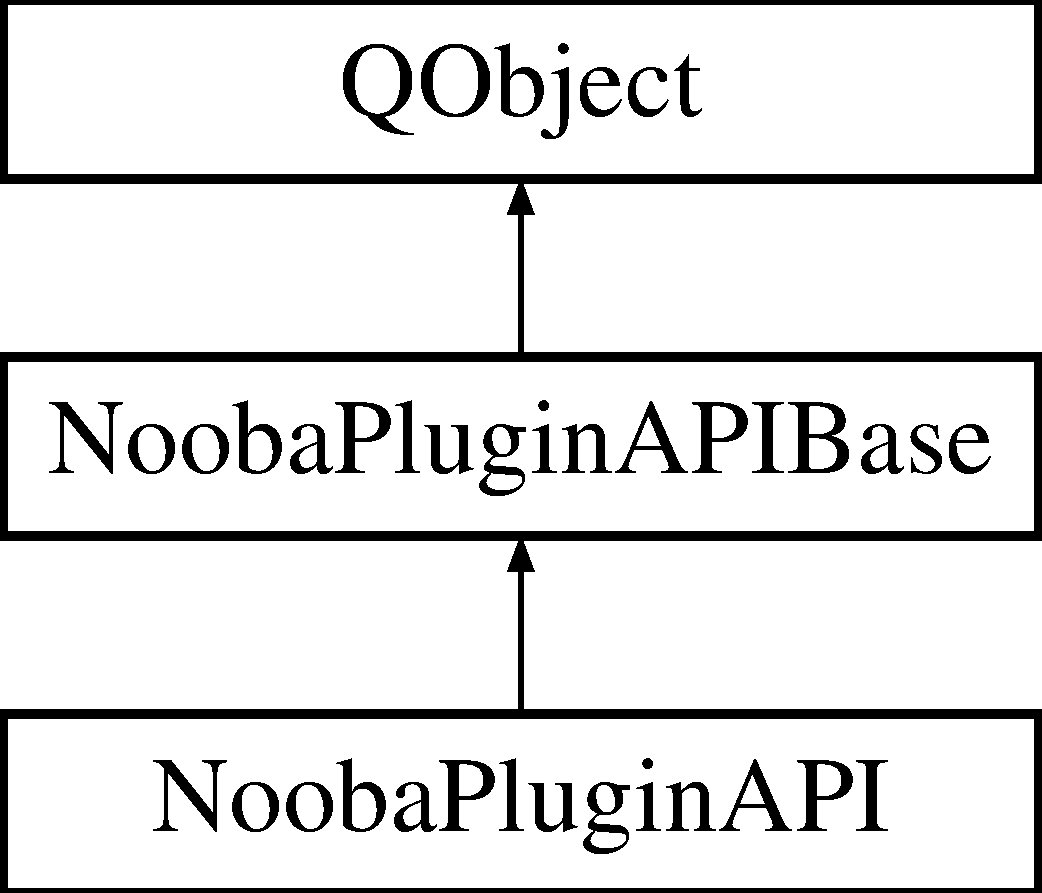
\includegraphics[height=3.000000cm]{class_nooba_plugin_a_p_i_base}
\end{center}
\end{figure}
\subsection*{Static Public Member Functions}
\begin{DoxyCompactItemize}
\item 
\hypertarget{class_nooba_plugin_a_p_i_base_a82408eedc0a13ec10c445c5e9441ecb7}{static int {\bfseries A\-P\-I\-Major\-Version} ()}\label{class_nooba_plugin_a_p_i_base_a82408eedc0a13ec10c445c5e9441ecb7}

\item 
\hypertarget{class_nooba_plugin_a_p_i_base_a75f0dfbe75dea5d77b38f83ec68d1bba}{static int {\bfseries A\-P\-I\-Minor\-Version} ()}\label{class_nooba_plugin_a_p_i_base_a75f0dfbe75dea5d77b38f83ec68d1bba}

\end{DoxyCompactItemize}


The documentation for this class was generated from the following files\-:\begin{DoxyCompactItemize}
\item 
/home/asitha/\-Documents/\-F\-Y\-P/\-Nooba\-V\-S\-S/\-Nooba\-Plugin\-A\-P\-I/noobapluginbase.\-h\item 
/home/asitha/\-Documents/\-F\-Y\-P/\-Nooba\-V\-S\-S/\-Nooba\-Plugin\-A\-P\-I/noobapluginbase.\-cpp\end{DoxyCompactItemize}

\hypertarget{class_nooba_plugin_a_p_i_base_private}{\section{Nooba\-Plugin\-A\-P\-I\-Base\-Private Class Reference}
\label{class_nooba_plugin_a_p_i_base_private}\index{Nooba\-Plugin\-A\-P\-I\-Base\-Private@{Nooba\-Plugin\-A\-P\-I\-Base\-Private}}
}
\subsection*{Public Member Functions}
\begin{DoxyCompactItemize}
\item 
\hypertarget{class_nooba_plugin_a_p_i_base_private_a1394e8b0fe3269b0996626445e35546c}{{\bfseries Nooba\-Plugin\-A\-P\-I\-Base\-Private} (\hyperlink{class_nooba_plugin_a_p_i_base}{Nooba\-Plugin\-A\-P\-I\-Base} $\ast$parent)}\label{class_nooba_plugin_a_p_i_base_private_a1394e8b0fe3269b0996626445e35546c}

\end{DoxyCompactItemize}
\subsection*{Public Attributes}
\begin{DoxyCompactItemize}
\item 
\hypertarget{class_nooba_plugin_a_p_i_base_private_a0952c0e27666aa2d8d62ca0ea246f07c}{\hyperlink{class_nooba_plugin_a_p_i_base}{Nooba\-Plugin\-A\-P\-I\-Base} $\ast$const {\bfseries q\-\_\-ptr}}\label{class_nooba_plugin_a_p_i_base_private_a0952c0e27666aa2d8d62ca0ea246f07c}

\end{DoxyCompactItemize}


The documentation for this class was generated from the following files\-:\begin{DoxyCompactItemize}
\item 
/home/asitha/\-Documents/\-F\-Y\-P/\-Nooba\-V\-S\-S/\-Nooba\-Plugin\-A\-P\-I/noobapluginbaseprivate.\-h\item 
/home/asitha/\-Documents/\-F\-Y\-P/\-Nooba\-V\-S\-S/\-Nooba\-Plugin\-A\-P\-I/noobapluginbaseprivate.\-cpp\end{DoxyCompactItemize}

\hypertarget{struct_nooba_plugin_a_p_i_private}{\section{Nooba\-Plugin\-A\-P\-I\-Private Struct Reference}
\label{struct_nooba_plugin_a_p_i_private}\index{Nooba\-Plugin\-A\-P\-I\-Private@{Nooba\-Plugin\-A\-P\-I\-Private}}
}


The \hyperlink{struct_nooba_plugin_a_p_i_private}{Nooba\-Plugin\-A\-P\-I\-Private} struct private data structure for \hyperlink{class_nooba_plugin_a_p_i}{Nooba\-Plugin\-A\-P\-I} class.  


\subsection*{Public Attributes}
\begin{DoxyCompactItemize}
\item 
\hypertarget{struct_nooba_plugin_a_p_i_private_aa45461d4401bdab4c21b4d4f2a074227}{Q\-String {\bfseries \-\_\-err\-Msg}}\label{struct_nooba_plugin_a_p_i_private_aa45461d4401bdab4c21b4d4f2a074227}

\end{DoxyCompactItemize}


\subsection{Detailed Description}
The \hyperlink{struct_nooba_plugin_a_p_i_private}{Nooba\-Plugin\-A\-P\-I\-Private} struct private data structure for \hyperlink{class_nooba_plugin_a_p_i}{Nooba\-Plugin\-A\-P\-I} class. 

The documentation for this struct was generated from the following file\-:\begin{DoxyCompactItemize}
\item 
/home/asitha/\-Documents/\-F\-Y\-P/\-Nooba\-V\-S\-S/\-Nooba\-Plugin\-A\-P\-I/noobapluginapi.\-cpp\end{DoxyCompactItemize}

\hypertarget{class_plugin_info}{\section{Plugin\-Info Class Reference}
\label{class_plugin_info}\index{Plugin\-Info@{Plugin\-Info}}
}


Plugin information are stored in this structure.  




{\ttfamily \#include $<$noobapluginapi.\-h$>$}

\subsection*{Public Member Functions}
\begin{DoxyCompactItemize}
\item 
\hypertarget{class_plugin_info_a28a7ce1796230a533b9bdb99653c9df5}{{\bfseries Plugin\-Info} (const Q\-String \&name, const int major\-Version, const int minor\-Version, const Q\-String \&description, const Q\-String \&author)}\label{class_plugin_info_a28a7ce1796230a533b9bdb99653c9df5}

\item 
\hypertarget{class_plugin_info_aab6b4739162eb44207b4854e19d3dd9d}{{\bfseries Plugin\-Info} (const \hyperlink{class_plugin_info}{Plugin\-Info} \&rhs)}\label{class_plugin_info_aab6b4739162eb44207b4854e19d3dd9d}

\item 
\hypertarget{class_plugin_info_aac1aba18706e202ebda5ea27de0e72f4}{\hyperlink{class_plugin_info}{Plugin\-Info} \& {\bfseries operator=} (const \hyperlink{class_plugin_info}{Plugin\-Info} \&rhs)}\label{class_plugin_info_aac1aba18706e202ebda5ea27de0e72f4}

\item 
\hypertarget{class_plugin_info_a1b864de6e5bfe9962c5cba713d35a84e}{Q\-String {\bfseries name} () const }\label{class_plugin_info_a1b864de6e5bfe9962c5cba713d35a84e}

\item 
\hypertarget{class_plugin_info_a0667c19893ce1bc822a096d18023e4ce}{Q\-String {\bfseries description} () const }\label{class_plugin_info_a0667c19893ce1bc822a096d18023e4ce}

\item 
\hypertarget{class_plugin_info_a9e8d357df9b02ef186799be731397cdb}{Q\-String {\bfseries author} () const }\label{class_plugin_info_a9e8d357df9b02ef186799be731397cdb}

\item 
\hypertarget{class_plugin_info_ab44ab9c20a907d7cc6aab3154e34d64a}{int {\bfseries major\-Version} () const }\label{class_plugin_info_ab44ab9c20a907d7cc6aab3154e34d64a}

\item 
\hypertarget{class_plugin_info_a0f81901bccba9544c180bd9eb813c0dc}{int {\bfseries minor\-Version} () const }\label{class_plugin_info_a0f81901bccba9544c180bd9eb813c0dc}

\end{DoxyCompactItemize}


\subsection{Detailed Description}
Plugin information are stored in this structure. 

The documentation for this class was generated from the following files\-:\begin{DoxyCompactItemize}
\item 
/home/asitha/\-Documents/\-F\-Y\-P/\-Nooba\-V\-S\-S/\-Nooba\-Plugin\-A\-P\-I/noobapluginapi.\-h\item 
/home/asitha/\-Documents/\-F\-Y\-P/\-Nooba\-V\-S\-S/\-Nooba\-Plugin\-A\-P\-I/noobapluginapi.\-cpp\end{DoxyCompactItemize}

\hypertarget{struct_plugin_info_private}{\section{Plugin\-Info\-Private Struct Reference}
\label{struct_plugin_info_private}\index{Plugin\-Info\-Private@{Plugin\-Info\-Private}}
}
\subsection*{Public Member Functions}
\begin{DoxyCompactItemize}
\item 
\hypertarget{struct_plugin_info_private_aa456adcfaa1bc3032c79a6bff88e21af}{{\bfseries Plugin\-Info\-Private} (const Q\-String \&name, const int major\-Version, const int minor\-Version, const Q\-String \&description, const Q\-String \&author)}\label{struct_plugin_info_private_aa456adcfaa1bc3032c79a6bff88e21af}

\end{DoxyCompactItemize}
\subsection*{Public Attributes}
\begin{DoxyCompactItemize}
\item 
\hypertarget{struct_plugin_info_private_a9aef39162eb012be3d0346c5bd4bee60}{Q\-String {\bfseries \-\_\-name}}\label{struct_plugin_info_private_a9aef39162eb012be3d0346c5bd4bee60}

\item 
\hypertarget{struct_plugin_info_private_a211871dfad64901e4d4a6e185eba46da}{Q\-String {\bfseries \-\_\-description}}\label{struct_plugin_info_private_a211871dfad64901e4d4a6e185eba46da}

\item 
\hypertarget{struct_plugin_info_private_a4811906914ca75ce88a83d5cfd6f0801}{Q\-String {\bfseries \-\_\-author}}\label{struct_plugin_info_private_a4811906914ca75ce88a83d5cfd6f0801}

\item 
\hypertarget{struct_plugin_info_private_ae9146c8770236fb182be9a902a332ae3}{int {\bfseries \-\_\-major\-Version}}\label{struct_plugin_info_private_ae9146c8770236fb182be9a902a332ae3}

\item 
\hypertarget{struct_plugin_info_private_a60f83bdde05cd0f91ba24d4f2f2ec308}{int {\bfseries \-\_\-minor\-Version}}\label{struct_plugin_info_private_a60f83bdde05cd0f91ba24d4f2f2ec308}

\end{DoxyCompactItemize}


The documentation for this struct was generated from the following file\-:\begin{DoxyCompactItemize}
\item 
/home/asitha/\-Documents/\-F\-Y\-P/\-Nooba\-V\-S\-S/\-Nooba\-Plugin\-A\-P\-I/noobapluginapi.\-cpp\end{DoxyCompactItemize}

\hypertarget{class_plugin_pass_data}{\section{Plugin\-Pass\-Data Class Reference}
\label{class_plugin_pass_data}\index{Plugin\-Pass\-Data@{Plugin\-Pass\-Data}}
}
\subsection*{Public Member Functions}
\begin{DoxyCompactItemize}
\item 
\hypertarget{class_plugin_pass_data_a1f1d979da0fabd694694080061fbacec}{\hyperlink{class_plugin_pass_data_a1f1d979da0fabd694694080061fbacec}{Plugin\-Pass\-Data} ()}\label{class_plugin_pass_data_a1f1d979da0fabd694694080061fbacec}

\begin{DoxyCompactList}\small\item\em \hyperlink{class_plugin_pass_data_a1f1d979da0fabd694694080061fbacec}{Plugin\-Pass\-Data\-::\-Plugin\-Pass\-Data}. \end{DoxyCompactList}\item 
\hypertarget{class_plugin_pass_data_a2b7fb9d514256481ede43828a6d87720}{{\bfseries Plugin\-Pass\-Data} (const \hyperlink{class_plugin_pass_data}{Plugin\-Pass\-Data} \&rhs)}\label{class_plugin_pass_data_a2b7fb9d514256481ede43828a6d87720}

\item 
\hypertarget{class_plugin_pass_data_a99626becacfee9af079074e1aee326e2}{\hyperlink{class_plugin_pass_data}{Plugin\-Pass\-Data} \& {\bfseries operator=} (const \hyperlink{class_plugin_pass_data}{Plugin\-Pass\-Data} \&rhs)}\label{class_plugin_pass_data_a99626becacfee9af079074e1aee326e2}

\item 
\hypertarget{class_plugin_pass_data_a9b30d96902dc5d5674779f4787b50f17}{Q\-String\-List {\bfseries str\-List} () const }\label{class_plugin_pass_data_a9b30d96902dc5d5674779f4787b50f17}

\item 
\hypertarget{class_plugin_pass_data_acb04c495ddea543c62b3dad2443c0244}{void {\bfseries set\-Str\-List} (const Q\-String\-List \&list)}\label{class_plugin_pass_data_acb04c495ddea543c62b3dad2443c0244}

\item 
\hypertarget{class_plugin_pass_data_a04a887d435f0821223014abe8670fa9e}{void {\bfseries append\-Str\-List} (const Q\-String \&str)}\label{class_plugin_pass_data_a04a887d435f0821223014abe8670fa9e}

\item 
\hypertarget{class_plugin_pass_data_a22e902d107d714dbac1ad37cfa4dde69}{void {\bfseries set\-Image} (const Q\-Image \&image)}\label{class_plugin_pass_data_a22e902d107d714dbac1ad37cfa4dde69}

\item 
\hypertarget{class_plugin_pass_data_aea26264180123c47956fdf2078a9912f}{Q\-Image \& {\bfseries get\-Image} () const }\label{class_plugin_pass_data_aea26264180123c47956fdf2078a9912f}

\end{DoxyCompactItemize}


The documentation for this class was generated from the following files\-:\begin{DoxyCompactItemize}
\item 
/home/asitha/\-Documents/\-F\-Y\-P/\-Nooba\-V\-S\-S/\-Nooba\-Plugin\-A\-P\-I/noobapluginapi.\-h\item 
/home/asitha/\-Documents/\-F\-Y\-P/\-Nooba\-V\-S\-S/\-Nooba\-Plugin\-A\-P\-I/noobapluginapi.\-cpp\end{DoxyCompactItemize}

\hypertarget{struct_plugin_pass_data_private}{\section{Plugin\-Pass\-Data\-Private Struct Reference}
\label{struct_plugin_pass_data_private}\index{Plugin\-Pass\-Data\-Private@{Plugin\-Pass\-Data\-Private}}
}


The \hyperlink{struct_plugin_pass_data_private}{Plugin\-Pass\-Data\-Private} struct.  


\subsection*{Public Attributes}
\begin{DoxyCompactItemize}
\item 
\hypertarget{struct_plugin_pass_data_private_a9dd4ebe057161144341ebd490a95ca96}{Q\-String\-List {\bfseries \-\_\-str\-List}}\label{struct_plugin_pass_data_private_a9dd4ebe057161144341ebd490a95ca96}

\item 
\hypertarget{struct_plugin_pass_data_private_a92c4dc9f66daef3b1a2550ecf5e2ecd1}{Q\-Image {\bfseries \-\_\-img}}\label{struct_plugin_pass_data_private_a92c4dc9f66daef3b1a2550ecf5e2ecd1}

\end{DoxyCompactItemize}


\subsection{Detailed Description}
The \hyperlink{struct_plugin_pass_data_private}{Plugin\-Pass\-Data\-Private} struct. 

The documentation for this struct was generated from the following file\-:\begin{DoxyCompactItemize}
\item 
/home/asitha/\-Documents/\-F\-Y\-P/\-Nooba\-V\-S\-S/\-Nooba\-Plugin\-A\-P\-I/noobapluginapi.\-cpp\end{DoxyCompactItemize}

\hypertarget{class_proc_params}{\section{Proc\-Params Class Reference}
\label{class_proc_params}\index{Proc\-Params@{Proc\-Params}}
}


Structure that uses to pass frame relevant data from the Frontend application to base plugin.  




{\ttfamily \#include $<$noobapluginapi.\-h$>$}

\subsection*{Public Member Functions}
\begin{DoxyCompactItemize}
\item 
\hypertarget{class_proc_params_a3d46f46584fcd75eae4204cf98fd1b31}{{\bfseries Proc\-Params} (const \hyperlink{class_proc_params}{Proc\-Params} \&rhs)}\label{class_proc_params_a3d46f46584fcd75eae4204cf98fd1b31}

\item 
\hypertarget{class_proc_params_a6237e03e1a2b7f521c79bfc448dcd48d}{\hyperlink{class_proc_params}{Proc\-Params} \& {\bfseries operator=} (const \hyperlink{class_proc_params}{Proc\-Params} \&rhs)}\label{class_proc_params_a6237e03e1a2b7f521c79bfc448dcd48d}

\item 
\hypertarget{class_proc_params_acf34cd3883991fbd99fb0843bcd023cd}{void {\bfseries set\-Frame\-Id} (int id)}\label{class_proc_params_acf34cd3883991fbd99fb0843bcd023cd}

\item 
\hypertarget{class_proc_params_a98e4f551be06dec588275aa5cd6e03bf}{int {\bfseries frame\-Id} () const }\label{class_proc_params_a98e4f551be06dec588275aa5cd6e03bf}

\item 
\hypertarget{class_proc_params_aacde091f2256f43d3029945d2cddeec1}{void {\bfseries set\-Frame\-Rate} (double rate)}\label{class_proc_params_aacde091f2256f43d3029945d2cddeec1}

\item 
\hypertarget{class_proc_params_a58c9adacf6f76b562d799945e8de9356}{double {\bfseries frame\-Rate} () const }\label{class_proc_params_a58c9adacf6f76b562d799945e8de9356}

\item 
\hypertarget{class_proc_params_a7a54dbb23763458d0d2563435d2e14a7}{void {\bfseries set\-Error\-State} (bool is\-Error)}\label{class_proc_params_a7a54dbb23763458d0d2563435d2e14a7}

\item 
\hypertarget{class_proc_params_a3bc8ac09ffc5f14fdbe7210027ae83db}{bool {\bfseries is\-Error} () const }\label{class_proc_params_a3bc8ac09ffc5f14fdbe7210027ae83db}

\item 
\hypertarget{class_proc_params_aeccfa47d9277cf2d2988b2b3eef596f4}{void {\bfseries set\-Error\-Msg} (const Q\-String \&err\-Msg)}\label{class_proc_params_aeccfa47d9277cf2d2988b2b3eef596f4}

\item 
\hypertarget{class_proc_params_a25a6f051c347283c9e1f9ee38a391369}{Q\-String {\bfseries err\-Msg} () const }\label{class_proc_params_a25a6f051c347283c9e1f9ee38a391369}

\item 
\hyperlink{namespacenooba_ae2951593fff55d4ea388efa06a663468}{nooba\-::\-Video\-State} \hyperlink{class_proc_params_ae2a581185d8020620661da189805617c}{current\-Video\-State} () const 
\begin{DoxyCompactList}\small\item\em current\-Video\-State gives the current video state \end{DoxyCompactList}\item 
bool \hyperlink{class_proc_params_a5f7f0b0285012242d8a0c492ccd1ff27}{set\-Vid\-State} (\hyperlink{namespacenooba_ae2951593fff55d4ea388efa06a663468}{nooba\-::\-Video\-State} state)
\begin{DoxyCompactList}\small\item\em set\-Video\-State Currently Nothing happens by calling this. Only changes the internal variable. No effect on the actual state. \end{DoxyCompactList}\end{DoxyCompactItemize}


\subsection{Detailed Description}
Structure that uses to pass frame relevant data from the Frontend application to base plugin. 

\subsection{Member Function Documentation}
\hypertarget{class_proc_params_ae2a581185d8020620661da189805617c}{\index{Proc\-Params@{Proc\-Params}!current\-Video\-State@{current\-Video\-State}}
\index{current\-Video\-State@{current\-Video\-State}!ProcParams@{Proc\-Params}}
\subsubsection[{current\-Video\-State}]{\setlength{\rightskip}{0pt plus 5cm}{\bf nooba\-::\-Video\-State} Proc\-Params\-::current\-Video\-State (
\begin{DoxyParamCaption}
{}
\end{DoxyParamCaption}
) const}}\label{class_proc_params_ae2a581185d8020620661da189805617c}


current\-Video\-State gives the current video state 

\begin{DoxyReturn}{Returns}

\end{DoxyReturn}
\hypertarget{class_proc_params_a5f7f0b0285012242d8a0c492ccd1ff27}{\index{Proc\-Params@{Proc\-Params}!set\-Vid\-State@{set\-Vid\-State}}
\index{set\-Vid\-State@{set\-Vid\-State}!ProcParams@{Proc\-Params}}
\subsubsection[{set\-Vid\-State}]{\setlength{\rightskip}{0pt plus 5cm}bool Proc\-Params\-::set\-Vid\-State (
\begin{DoxyParamCaption}
\item[{{\bf nooba\-::\-Video\-State}}]{state}
\end{DoxyParamCaption}
)}}\label{class_proc_params_a5f7f0b0285012242d8a0c492ccd1ff27}


set\-Video\-State Currently Nothing happens by calling this. Only changes the internal variable. No effect on the actual state. 


\begin{DoxyParams}{Parameters}
{\em state} & \\
\hline
\end{DoxyParams}
\begin{DoxyReturn}{Returns}
bool setting the video state was sucessful or not 
\end{DoxyReturn}


The documentation for this class was generated from the following files\-:\begin{DoxyCompactItemize}
\item 
/home/asitha/\-Documents/\-F\-Y\-P/\-Nooba\-V\-S\-S/\-Nooba\-Plugin\-A\-P\-I/noobapluginapi.\-h\item 
/home/asitha/\-Documents/\-F\-Y\-P/\-Nooba\-V\-S\-S/\-Nooba\-Plugin\-A\-P\-I/noobapluginapi.\-cpp\end{DoxyCompactItemize}

\hypertarget{struct_proc_params_private}{\section{Proc\-Params\-Private Struct Reference}
\label{struct_proc_params_private}\index{Proc\-Params\-Private@{Proc\-Params\-Private}}
}
\subsection*{Public Attributes}
\begin{DoxyCompactItemize}
\item 
\hypertarget{struct_proc_params_private_abf93f72a095a036e15cde96a06ad4543}{bool {\bfseries \-\_\-is\-Error}}\label{struct_proc_params_private_abf93f72a095a036e15cde96a06ad4543}

\item 
\hypertarget{struct_proc_params_private_a42b05bcd78f019df67b0d33f3b1b45d4}{\hyperlink{namespacenooba_ae2951593fff55d4ea388efa06a663468}{nooba\-::\-Video\-State} {\bfseries \-\_\-current\-State}}\label{struct_proc_params_private_a42b05bcd78f019df67b0d33f3b1b45d4}

\item 
\hypertarget{struct_proc_params_private_a7c40008e121da968d06f5db84552a078}{int {\bfseries \-\_\-frame\-Id}}\label{struct_proc_params_private_a7c40008e121da968d06f5db84552a078}

\item 
\hypertarget{struct_proc_params_private_af3a49c173c14ce1be21d7289379395ff}{double {\bfseries \-\_\-frame\-Rate}}\label{struct_proc_params_private_af3a49c173c14ce1be21d7289379395ff}

\item 
\hypertarget{struct_proc_params_private_afd4955dfad038918e2be4580b9441f2b}{Q\-String {\bfseries \-\_\-err\-Msg}}\label{struct_proc_params_private_afd4955dfad038918e2be4580b9441f2b}

\end{DoxyCompactItemize}


The documentation for this struct was generated from the following file\-:\begin{DoxyCompactItemize}
\item 
/home/asitha/\-Documents/\-F\-Y\-P/\-Nooba\-V\-S\-S/\-Nooba\-Plugin\-A\-P\-I/noobapluginapi.\-cpp\end{DoxyCompactItemize}

\addcontentsline{toc}{part}{Index}
\printindex
\end{document}
